\section{Ein Beispiel zum rechnen und nachbauen}

\begin{frame}{Das System}
  \begin{figure}
    \caption{Eine Hand kann in das System gehalten werden und der Hintergrund ist weiterhin zu sehen.}
    \centering
    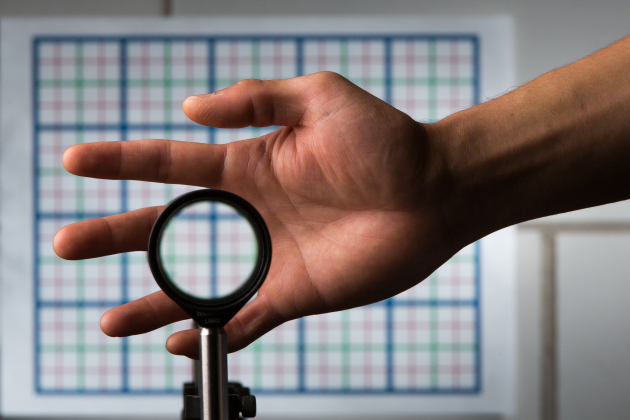
\includegraphics[height=0.6\textheight]{images/hand-cloak.jpg}
  \end{figure}
  Die folgenden Folien beziehen sich auf
  \href{https://www.rochester.edu/newscenter/watch-rochester-cloak-uses-ordinary-lenses-to-hide-objects-across-continuous-range-of-angles-70592/}{diese Veröffentlichung},
  und das zugeh\"orige Paper das verlinkt ist,
  von Howell und Choi der Universität Rochester aus dem Jahr 2014.
\end{frame}

\subsection{Einschub: Matrizenoptik}
\begin{frame}{Matrizenoptik}
  \begin{columns}
    \begin{column}{0.48\textwidth}
      \begin{figure}
        \centering
        \caption{Das System in Seitenansicht.}
        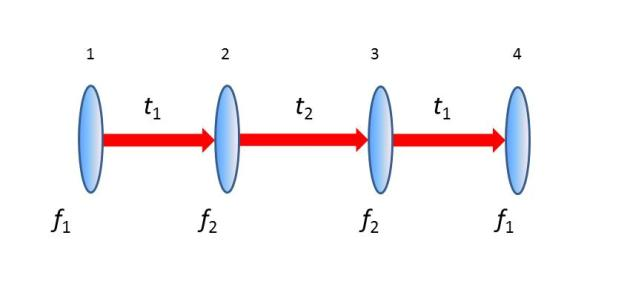
\includegraphics[width=\textwidth]{images/linsen.jpg}
      \end{figure}
    \end{column}
    \begin{column}{0.48\textwidth}
      D\"unne Linse
      \begin{align*}
        F_i &=
        \begin{pmatrix}
          1 & 0 \\
          -\frac{1}{f_i} & 1 \\
        \end{pmatrix}
        \intertext{Translation}
        T_i &=
        \begin{pmatrix}
          1 & t_i \\
          0 & 1 \\
        \end{pmatrix}
      \end{align*}
    \end{column}
  \end{columns}
\end{frame}

\begin{frame}{Matrizenoptik - Grundlagen}
  Annahmen der Matrizenoptik:
  \begin{enumerate}
    \item $λ\:<\!<$ alle Abmessungen des Systems $\to$ geometrische Optik
    \item axialsymmetrische Strahlen
    \item achsennahe Strahlen: $\sin(α) \approx \tan(α) \approx α$
  \end{enumerate}
  \pause
  \begin{columns}
    \begin{column}{0.4\textwidth}
      Beschreibung der Strahlen durch
      \begin{align*}
        \text{Achsenabstand}\;&y \\
        \text{Steigung}\;&v
        \intertext{Betrachtung des Brechungsindizes $n$:}
        V &\coloneq nv \\
        t &\coloneq \frac{x}{n}
      \end{align*}
    \end{column}
    \begin{column}{0.58\textwidth}
      Translationsmatrix:
      \begin{align*}
        \begin{pmatrix} y_2 \\ v_2 \\ \end{pmatrix} =
        \begin{pmatrix} 1 & x \\ 0 & 1 \\ \end{pmatrix}
        \begin{pmatrix} y_1 \\ v_1 \\ \end{pmatrix}
        &\implies
        \begin{pmatrix} Y_2 \\ V_2 \\ \end{pmatrix} =
        \begin{pmatrix} 1 & t \\ 0 & 1 \\ \end{pmatrix}
        \begin{pmatrix} Y_1 \\ V_1 \\ \end{pmatrix}
        \intertext{Refraktionsmatrix (d\"unne Linsen):}
        F = \begin{pmatrix} 1 & 0 \\ -\frac{n_2-n_1}{r} & 1 \\ \end{pmatrix}
        &\implies \begin{pmatrix} 1 & 0 \\ -P & 1 \\ \end{pmatrix}
        = \begin{pmatrix} 1 & 0 \\ -\frac{1}{f} & 1 \\ \end{pmatrix} \\
        f &: \text{Brennweite}
      \end{align*}
    \end{column}
  \end{columns}
\end{frame}

\subsection{Rechnungen}
\begin{frame}{Warum vier Linsen?}
  Eine Tarnkappe der L\"ange $L$ wird in der Matrizenoptik durch
  \begin{align*}
    M_\text{tarn} &=
    \begin{pmatrix}
      1 & L \\
      0 & 1 \\
    \end{pmatrix}
    =
    \begin{pmatrix}
      A & B \\
      C & D \\
    \end{pmatrix}
    \intertext{dargestellt. Eine Linse kann diese Bedingung nur erfüllen, wenn}
    M_{L=1} &=
    \begin{pmatrix}
      1 & 0 \\
      -\frac{1}{f_1} & 1 \\
    \end{pmatrix} = M_\text{tarn}
    \intertext{gilt, also}
    f_1 &\to \infty\:.
  \end{align*}
  Das entspricht einer Glasscheibe.
\end{frame}

\begin{frame}{Zwei Linsen}
  Die Gleichung f\"ur zwei Linsen lautet
  \begin{align*}
    M_{L=2} &= F_2\:T_1\:F_1 =
    \begin{pmatrix}
      1-\frac{t_1}{f_1} & t_1 \\
      -\frac{f_1+f_2-t_1}{f_1f_2} & 1-\frac{t_1}{f_2} \\
    \end{pmatrix}
    \stackrel{!}{=}
    \begin{pmatrix} A & B \\ C & D \\ \end{pmatrix} =
    \begin{pmatrix} 1 & L \\ 0 & 1 \\ \end{pmatrix}
    \intertext{Daraus folgt}
    \begin{drcases}
      t_1 = L = 0 \\
      f_1 \to \infty \\
      f_2 \to \infty
    \end{drcases}
    &=
    \begin{pmatrix}
      1 & 0 \\
      0 & 1 \\
    \end{pmatrix}
  \end{align*}
\end{frame}

\begin{frame}{Erweiterung auf drei Linsen}
  \begin{equation*}
    M_{L=3} = F_3\:T_2\:M_{L=2} = \frac{1}{f_2}
    \begin{pmatrix}
      \frac{f_1f_2-t_1f_2-t_2f_2-t_2f_1+t_1t_2}{f_1} & t_1f_2-t_1t_2+t_2f_2 \\
      -\frac{f_1f_2+f_2f_3-t_1f_2-t_2f_2+f_1f_3-t_1f_3-t_2f_1+t_1t_2}{f_1f_3}
      & \frac{f_2f_3-t_1f_3-t_1f_2-t_2f_2+t_1t_2}{f_3} \\
    \end{pmatrix}
    \stackrel{!}{=}
    \begin{pmatrix} A & B \\ C & D \\ \end{pmatrix} =
    \begin{pmatrix} 1 & L \\ 0 & 1 \\ \end{pmatrix}
  \end{equation*}
  Es ergeben sich durch die Bedingungen einer Tarnkappe:
  \begin{columns}
    \begin{column}{0.32\textwidth}
      \begin{align*}
        C &= 0 \\
        f_2 &= -\frac{(f_3-t_2)(f_1-t_1)}{f_1+f_3-t_1-t_2}
      \end{align*}
    \end{column}
    \begin{column}{0.32\textwidth}
      \begin{align*}
        B &= L = t_1 + t_2 - \frac{t_1t_2}{f_2} \\
        0 &= t_1 t_2 \frac{f_1+f_3-t_1-t_2}{(f_3-t_2)(f_1-t_1)}\\
        &\implies t_1 = 0\;\text{v}\;t_2 = 0 \\
        &\text{v}\;f_1+f_3-t_1-t_2 = 0
      \end{align*}
    \end{column}
    \begin{column}{0.32\textwidth}
      \begin{align*}
        f_1 &= f_3 \;\wedge\; t_1 = t_2 \\
        f_2 &= \frac{t_1-f_1}{2}
      \end{align*}
      mit $f_1>\!>t_1$ $\implies$ Tarnkappe
    \end{column}
  \end{columns}
\end{frame}

\begin{frame}{Schließlich das System mit allen vier Linsen}
  \begin{columns}
    \begin{column}{0.48\textwidth}
      Zuerst ein paar Annahmen:
      \begin{align*}
        f_1 &= f_4 \\
        f_2 &= f_3 \\
        t_1 &= t_3
        \intertext{Stellen wir nun die Matrizen auf:}
        M_{L=4} &= F_4\:T_3\:F_3\:T_2\:F_2\:T_1\:F_1 \\
        &= F_1\:T_1\:F_2\:T_2\:F_2\:T_1\:F_1
        \intertext{als zus\"atzliche Bedingung nehmen wir an:}
        t_1 &= f_1 + f_2
      \end{align*}
    \end{column}
    \begin{column}{0.48\textwidth}
      Damit vereinfacht sich die Matrix zu:
      \begin{align*}
        M_{L=4} &=
        \begin{pmatrix}
          1 & \frac{f_1^2t_2}{f_2^2}-\frac{2f_1^2}{f_2}-2f_1 \\
          0 & 1 \\
        \end{pmatrix}
        \stackrel{!}{=}
        \begin{pmatrix} 1 & L \\ 0 & 1 \\ \end{pmatrix} \\~\\
        L &= 2t_1 + t_2 = 2f_1 + 2f_2 + t_2 \\
        \implies\;t_2 &= -2f_2 \frac{f_1+f_2}{f_1-f_2} \\
        &\implies\;f_2 > f_1
      \end{align*}
    \end{column}
  \end{columns}  
\end{frame}

\subsection{Aufbau}
\begin{frame}{Wechsel von der Theorie in die Praxis}
  \begin{figure}
    \centering
    \caption{Frontansicht mit Joseph Chai, \cite{rochester}}
    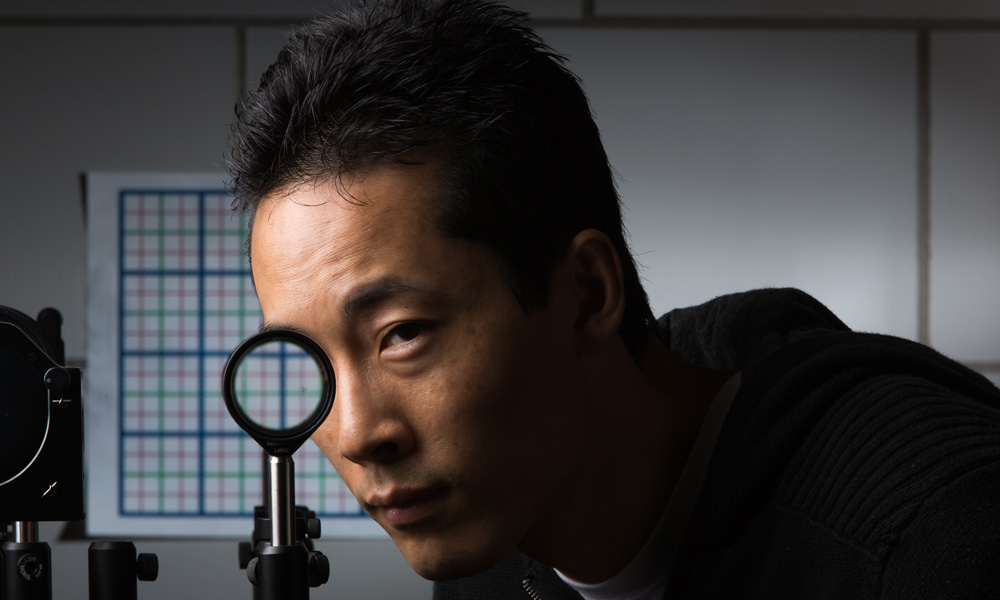
\includegraphics[height=0.8\textheight]{images/auge.jpg}
  \end{figure}
  
\end{frame}

\begin{frame}{Gibt es eine Winkelabh\"angigkeit?}
  \begin{columns}
    \begin{column}{0.49\textwidth}
      \begin{align*}
        f_1 &= \SI{200}{\milli\meter} \\
        f_2 &= \SI{75}{\milli\meter}
        \intertext{Winkel bez\"uglich der Mittelachse:}
        (a) \quad &\SI{-0.65}{\degree} \\ 
        (b) \quad &\SI{0}{\degree} \\ 
        (c) \quad &\SI{0.47}{\degree} \\ 
        (d) \quad &\SI{0.95}{\degree} \\
        ~&~ \\
        \text{Abstand: Schirm-Linse} \quad &\SI{1.9}{\meter} \\
        \text{Abstand: Linse-Kamera} \quad &\SI{3.1}{\meter}
      \end{align*}
    \end{column}
    \begin{column}{0.5\textwidth}
      \begin{figure}
        \centering
        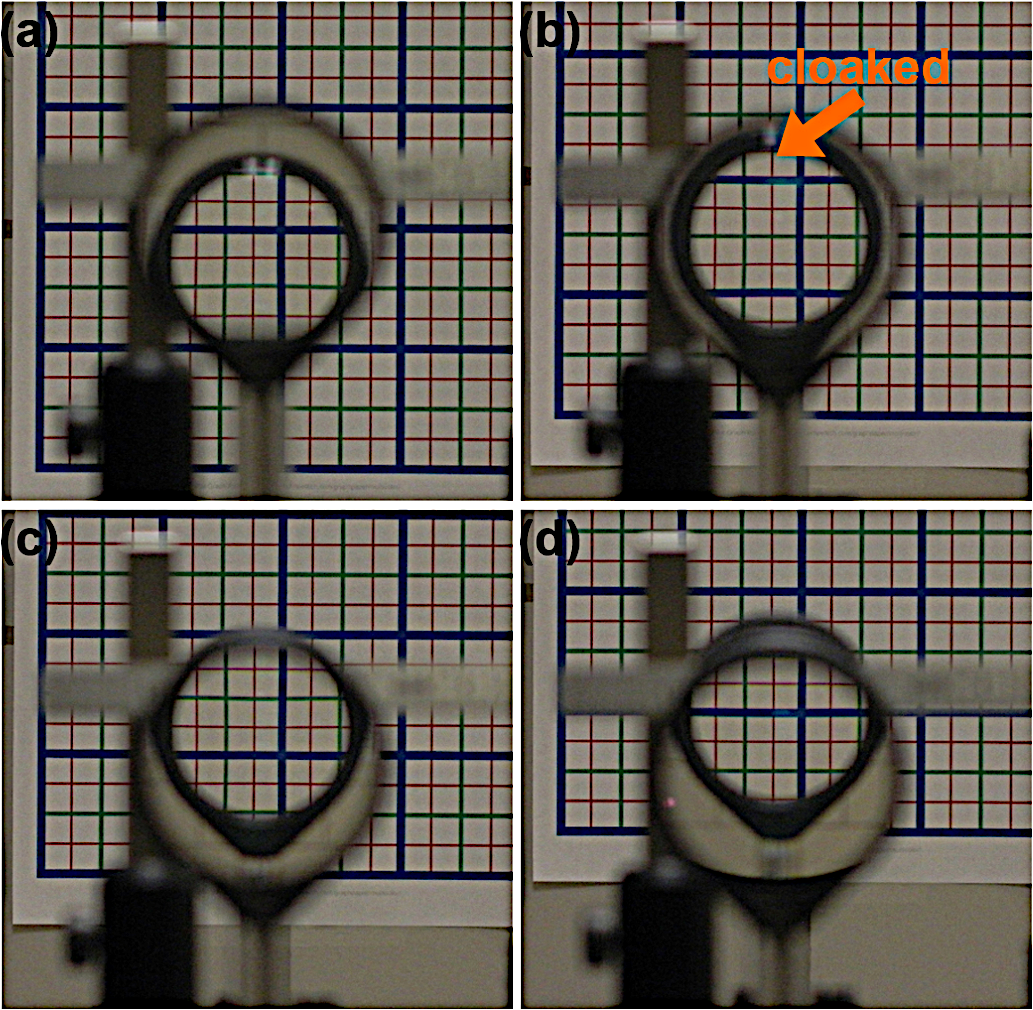
\includegraphics[height=0.8\textheight]{images/winkel.png}
      \end{figure}
    \end{column}
  \end{columns}
\end{frame}

\begin{frame}{Weclher Bereich wird getarnt?}
  \begin{figure}
    \centering
    \caption{Simulation der Lichtstrahlen durch das Linsensystem.}
    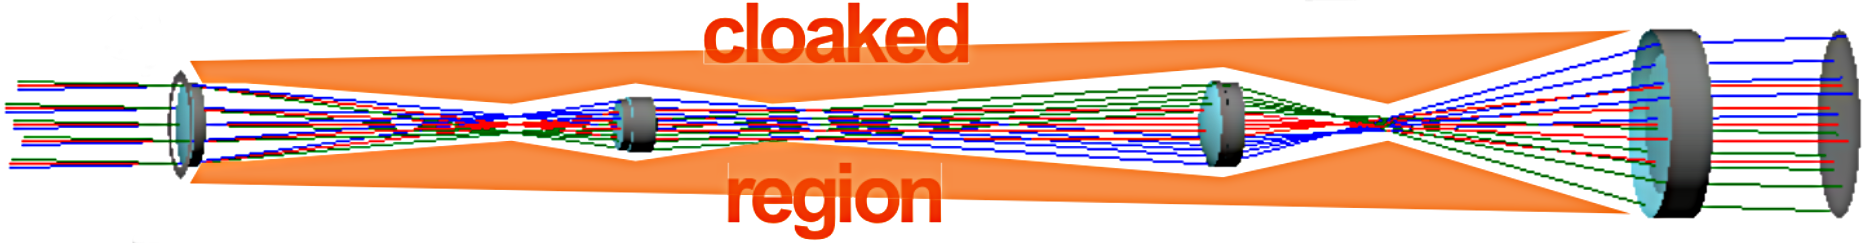
\includegraphics[width=0.8\textwidth]{images/skizze.png}
  \end{figure}
  \begin{figure}
    \centering
    \caption{Seitenaufnahme des Linsensystems.}
    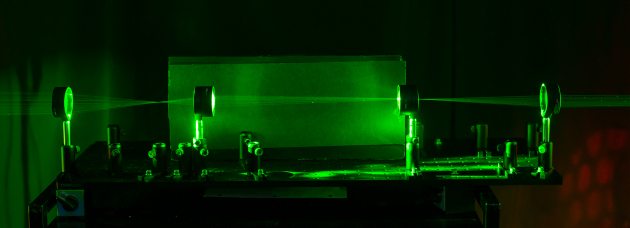
\includegraphics[width=0.6\textwidth]{images/laser-seite.jpg}
  \end{figure}

\end{frame}
\subsection{Anwendungen}
\begin{frame}{M\"ogliche Anwendungen}
  \begin{itemize}
    \item Durchschauen der H\"ande
      \begin{itemize}
        \item Chirurg
        \item Mechaniker
      \end{itemize}
    \item Verkleinern von toten Winkeln, z.B. bei LKWs
    \item tarnen von Kabeln bei Messaufbauten, oder anderen Ger\"aten
  \end{itemize}
\end{frame}
